\chapter{Pruebas y resultados}\label{cap:pruebas}

Este capítulo documenta las pruebas experimentales realizadas para la
caracterización y validación de los subsistemas del biorreactor. Los resultados
obtenidos fueron determinantes para la sintonización de los controladores previamente descritos en la Sección~\ref{cap8}.

% ---------------------------------------------------------------
\section{Ensamble del biorreactor}
% ---------------------------------------------------------------

En la Figura~\ref{fig:bio_interior_difusor} se muestra la construcción de
la estructura inferior del biorreactor junto con su pasamuro correspondiente,
el burbujeador y el oring, mientras que en las
Figuras~\ref{fig:bio_cuerpo_lateral} y~\ref{fig:bio_downcomer_codo} se
muestran las piezas finales de la estructura intermedia y la estructura
superior del biorreactor. Finalmente, en la
Figura~\ref{fig:bio_ensamble_sensores} se muestra el biorreactor ensamblado
con todos sus componentes.

\begin{figure}[H]
  \centering
  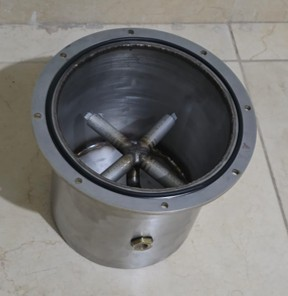
\includegraphics[width=0.50\textwidth]{Figuras/bio_interior_difusor}
  \caption{Parte inferior del biorreactor con el pasamuros y burbujeador.}
  \label{fig:bio_interior_difusor}
\end{figure}

\begin{figure}[H]
  \centering
  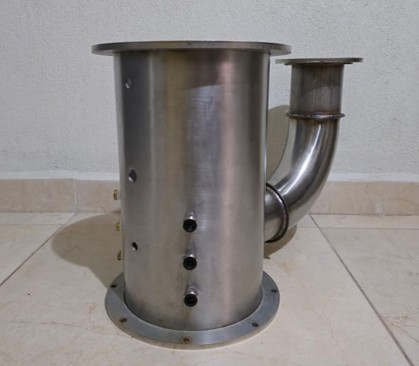
\includegraphics[width=0.50\textwidth]{Figuras/bio_cuerpo_lateral}
  \caption{Parte intermedia del biorreactor.}
  \label{fig:bio_cuerpo_lateral}
\end{figure}

\begin{figure}[H]
  \centering
  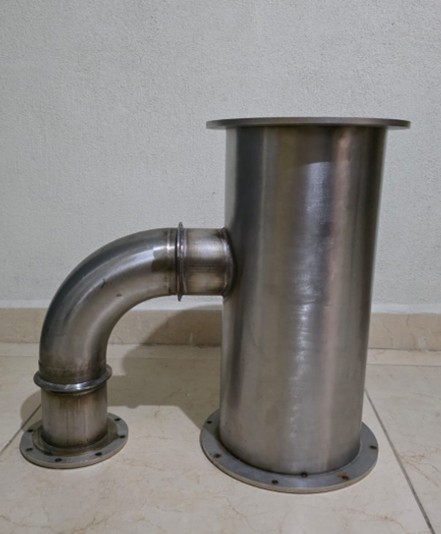
\includegraphics[width=0.50\textwidth]{Figuras/bio_downcomer_codo}
  \caption{Parte superior del biorreactor.}
  \label{fig:bio_downcomer_codo}
\end{figure}

\begin{figure}[H]
  \centering
  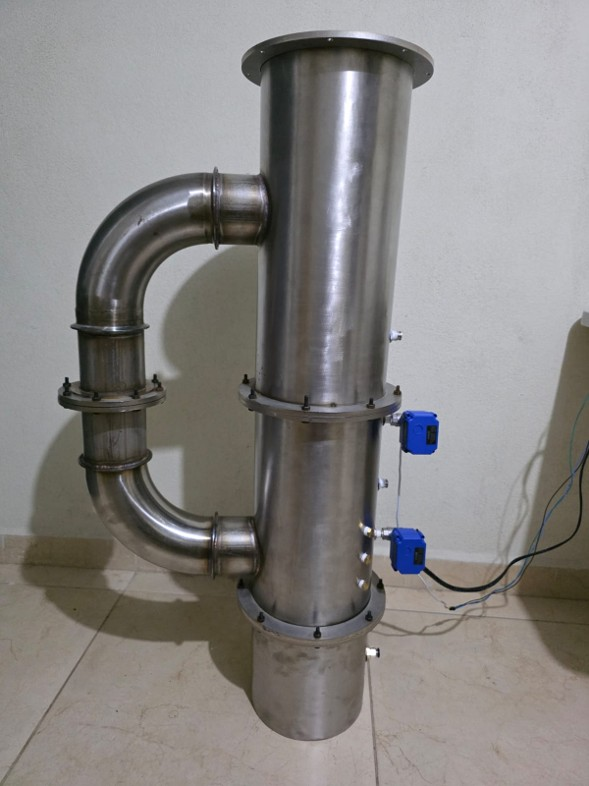
\includegraphics[width=0.65\textwidth]{Figuras/bio_ensamble_sensores}
  \caption{Biorreactor ensamblado con sensores instalados.}
  \label{fig:bio_ensamble_sensores}
\end{figure}

En la Figura~\ref{fig:bio_burbujeo_superior} se muestra el funcionamiento
del sistema de burbujeo únicamente con la parte inferior del biorreactor,
comprobando la correcta distribución de aire antes del ensamble final.

\begin{figure}[H]
  \centering
  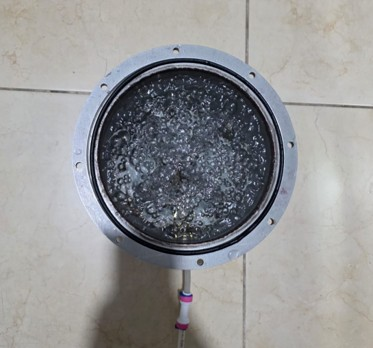
\includegraphics[width=0.50\textwidth]{Figuras/bio_burbujeo_superior}
  \caption{Comprobación del correcto funcionamiento del sistema de burbujeo.}
  \label{fig:bio_burbujeo_superior}
\end{figure}

En la Figura~\ref{fig:hmi_interior_cableado} se muestran las conexiones
eléctricas internas de los componentes para el funcionamiento de la HMI,
mientras que en la Figura~\ref{fig:hmi_panel_altavoces} se muestra la tapa
superior de manera invertida, en la cual se puede apreciar el soporte para
la pantalla así como las bocinas del sistema de sonido. Finalmente, en las
Figuras~\ref{fig:hmi_exterior_lateral} y~\ref{fig:hmi_panel_conectores} se
muestra la HMI ensamblada desde su vista frontal y trasera respectivamente.

\begin{figure}[H]
  \centering
  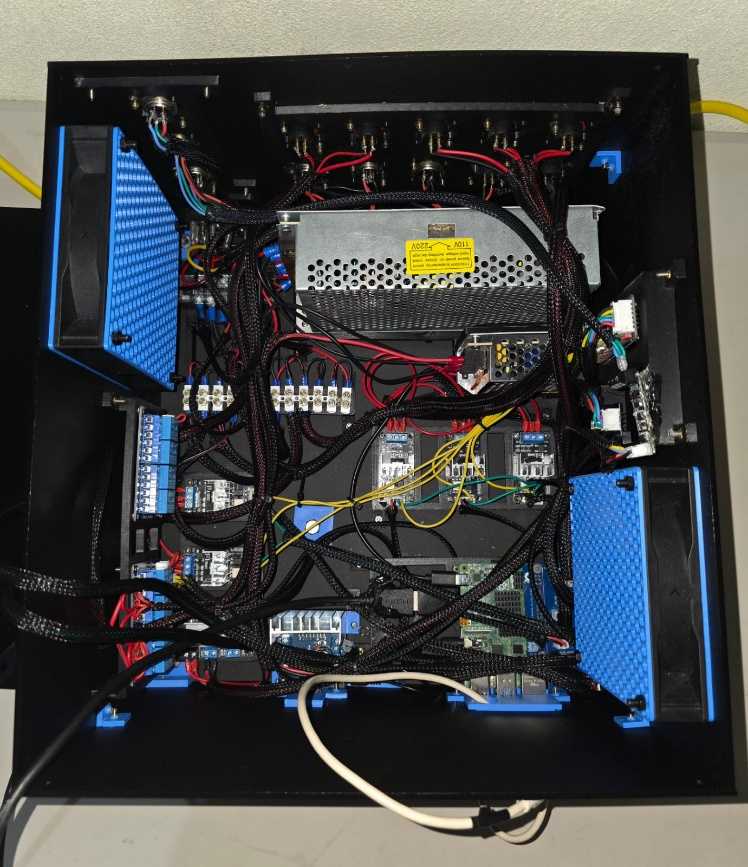
\includegraphics[width=0.85\textwidth]{Figuras/hmi_interior_cableado}
  \caption{Conexiones eléctricas internas de la HMI.}
  \label{fig:hmi_interior_cableado}
\end{figure}

\begin{figure}[H]
  \centering
  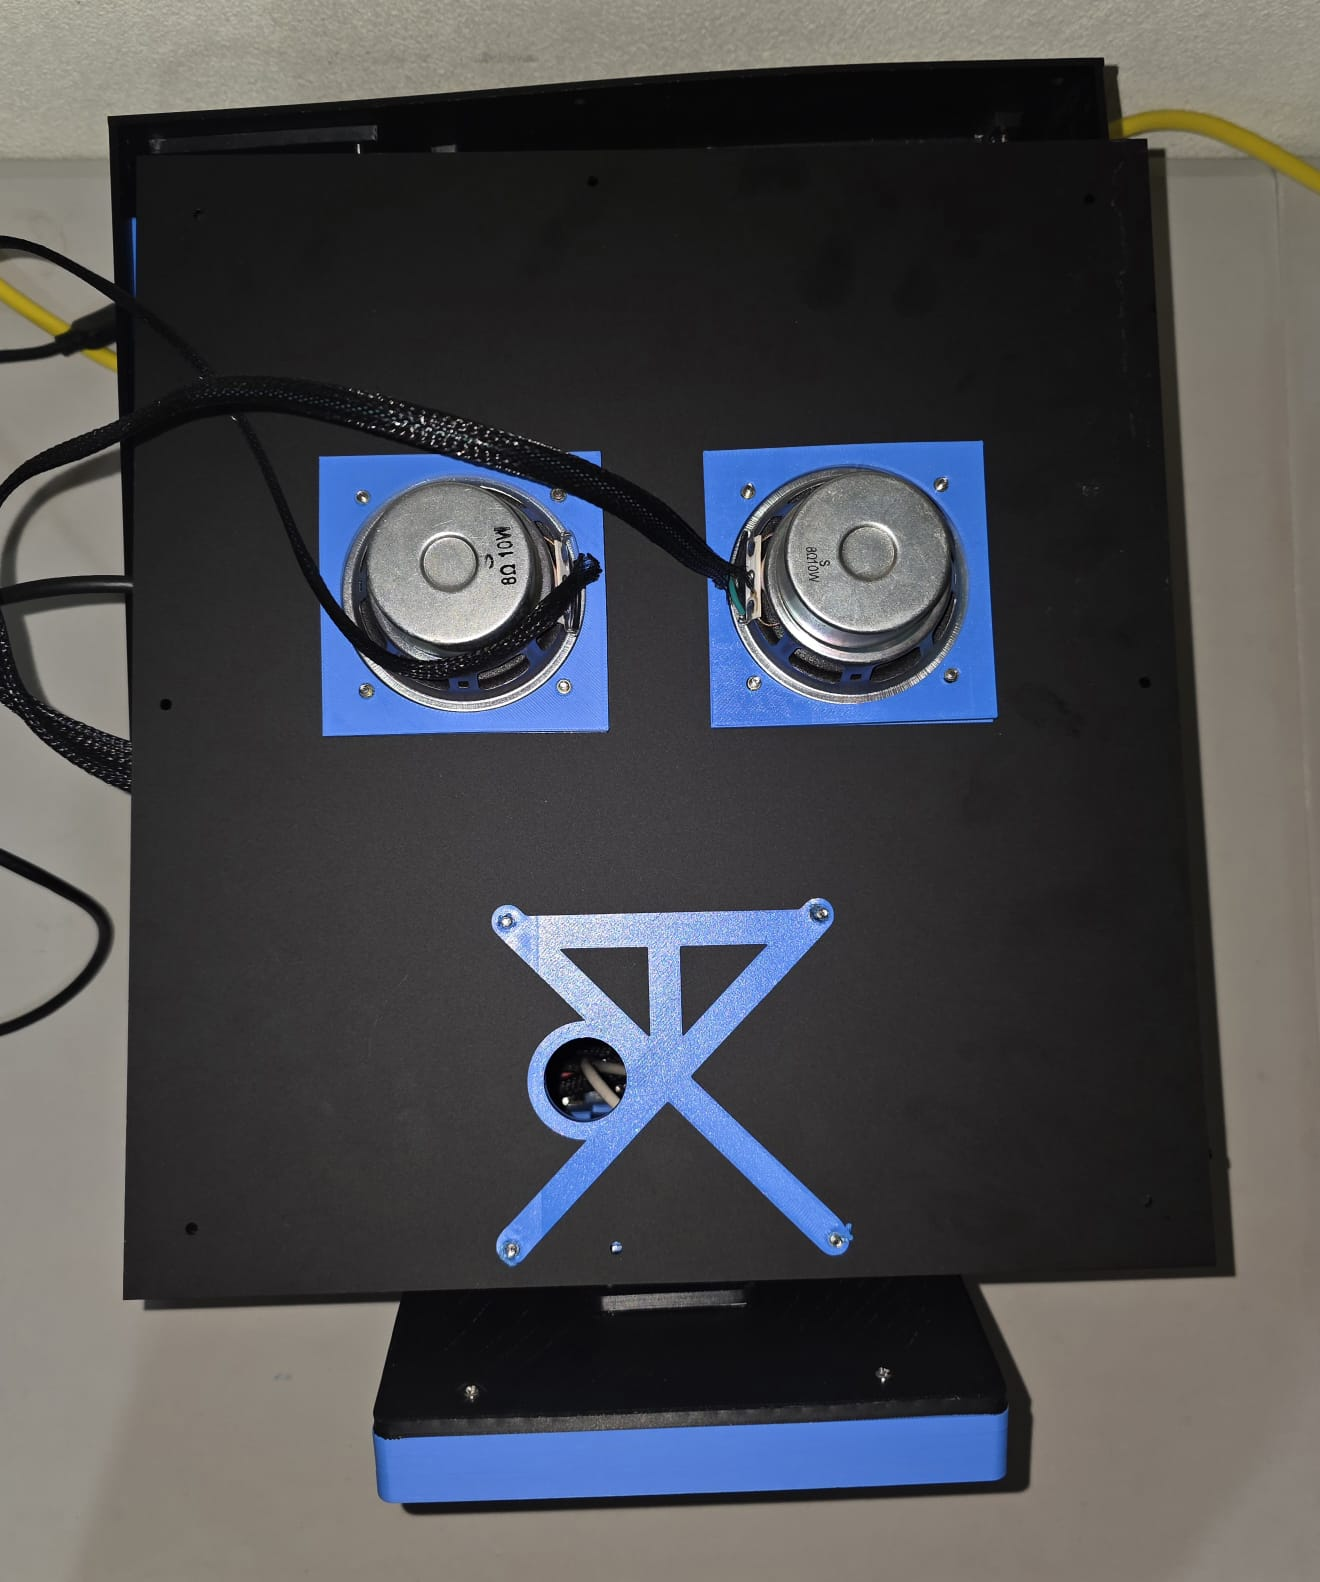
\includegraphics[width=0.60\textwidth]{Figuras/hmi_panel_altavoces}
  \caption{Tapadera de la HMI invertida mostrando soportes de bocinas y pantalla.}
  \label{fig:hmi_panel_altavoces}
\end{figure}

\begin{figure}[H]
  \centering
  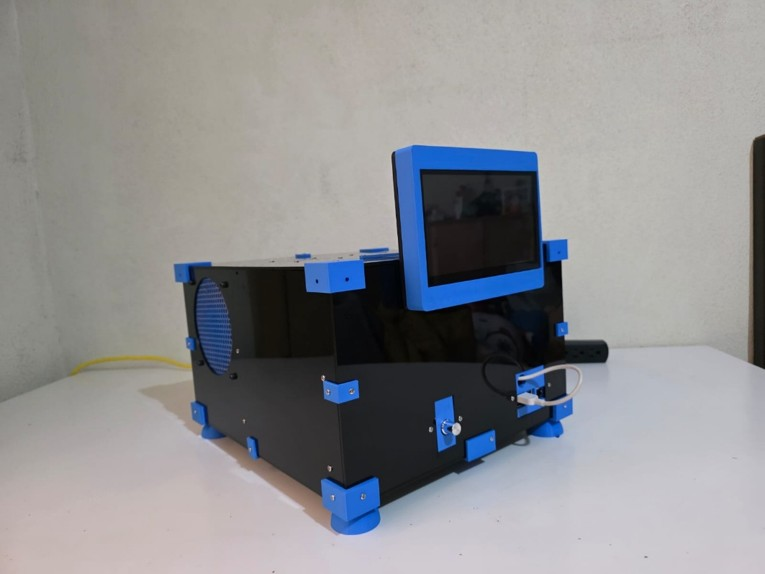
\includegraphics[width=0.75\textwidth]{Figuras/hmi_exterior_lateral}
  \caption{HMI ensamblada.}
  \label{fig:hmi_exterior_lateral}
\end{figure}

\begin{figure}[H]
  \centering
  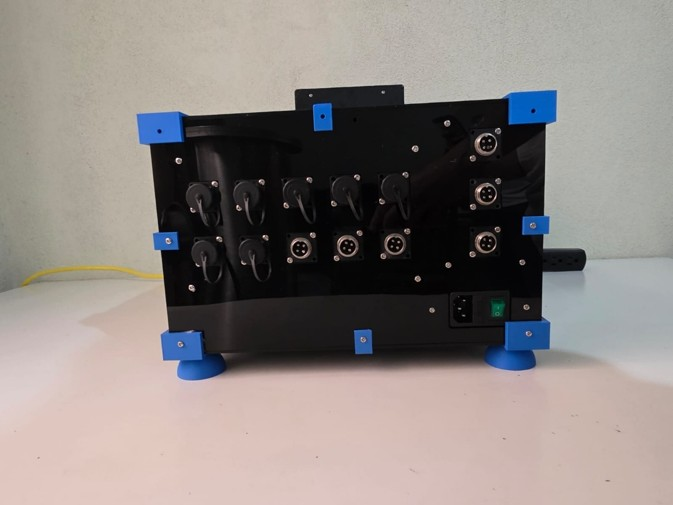
\includegraphics[width=0.75\textwidth]{Figuras/hmi_panel_conectores}
  \caption{Parte posterior de la HMI con la pared de conexiones.}
  \label{fig:hmi_panel_conectores}
\end{figure}

En la Figura~\ref{fig:bio_modulo_bombas} se muestra la lámina de soporte
para las bombas magnéticas de agua y la bomba de aire.

\begin{figure}[H]
  \centering
  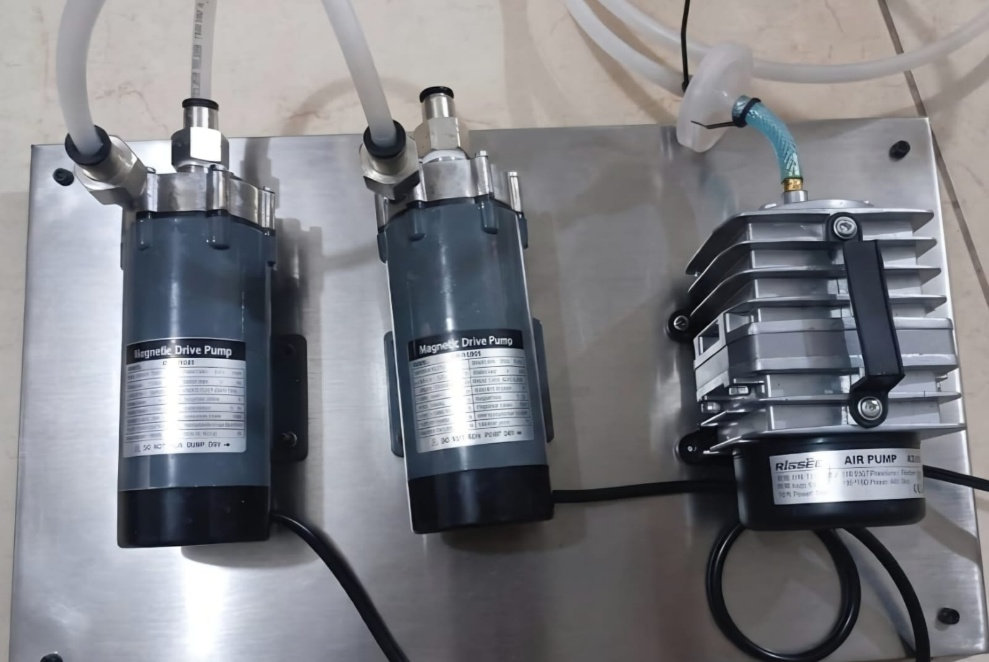
\includegraphics[width=0.85\textwidth]{Figuras/bio_modulo_bombas}
  \caption{Lámina de soporte de las bombas de agua y aire.}
  \label{fig:bio_modulo_bombas}
\end{figure}

Por último, en la Figura~\ref{fig:sistema_completo} se muestra el conjunto
de componentes que conforman el sistema del biorreactor: el biorreactor con
sus sensores, la HMI y el módulo de bombas de agua y aire.

\begin{figure}[H]
  \centering
  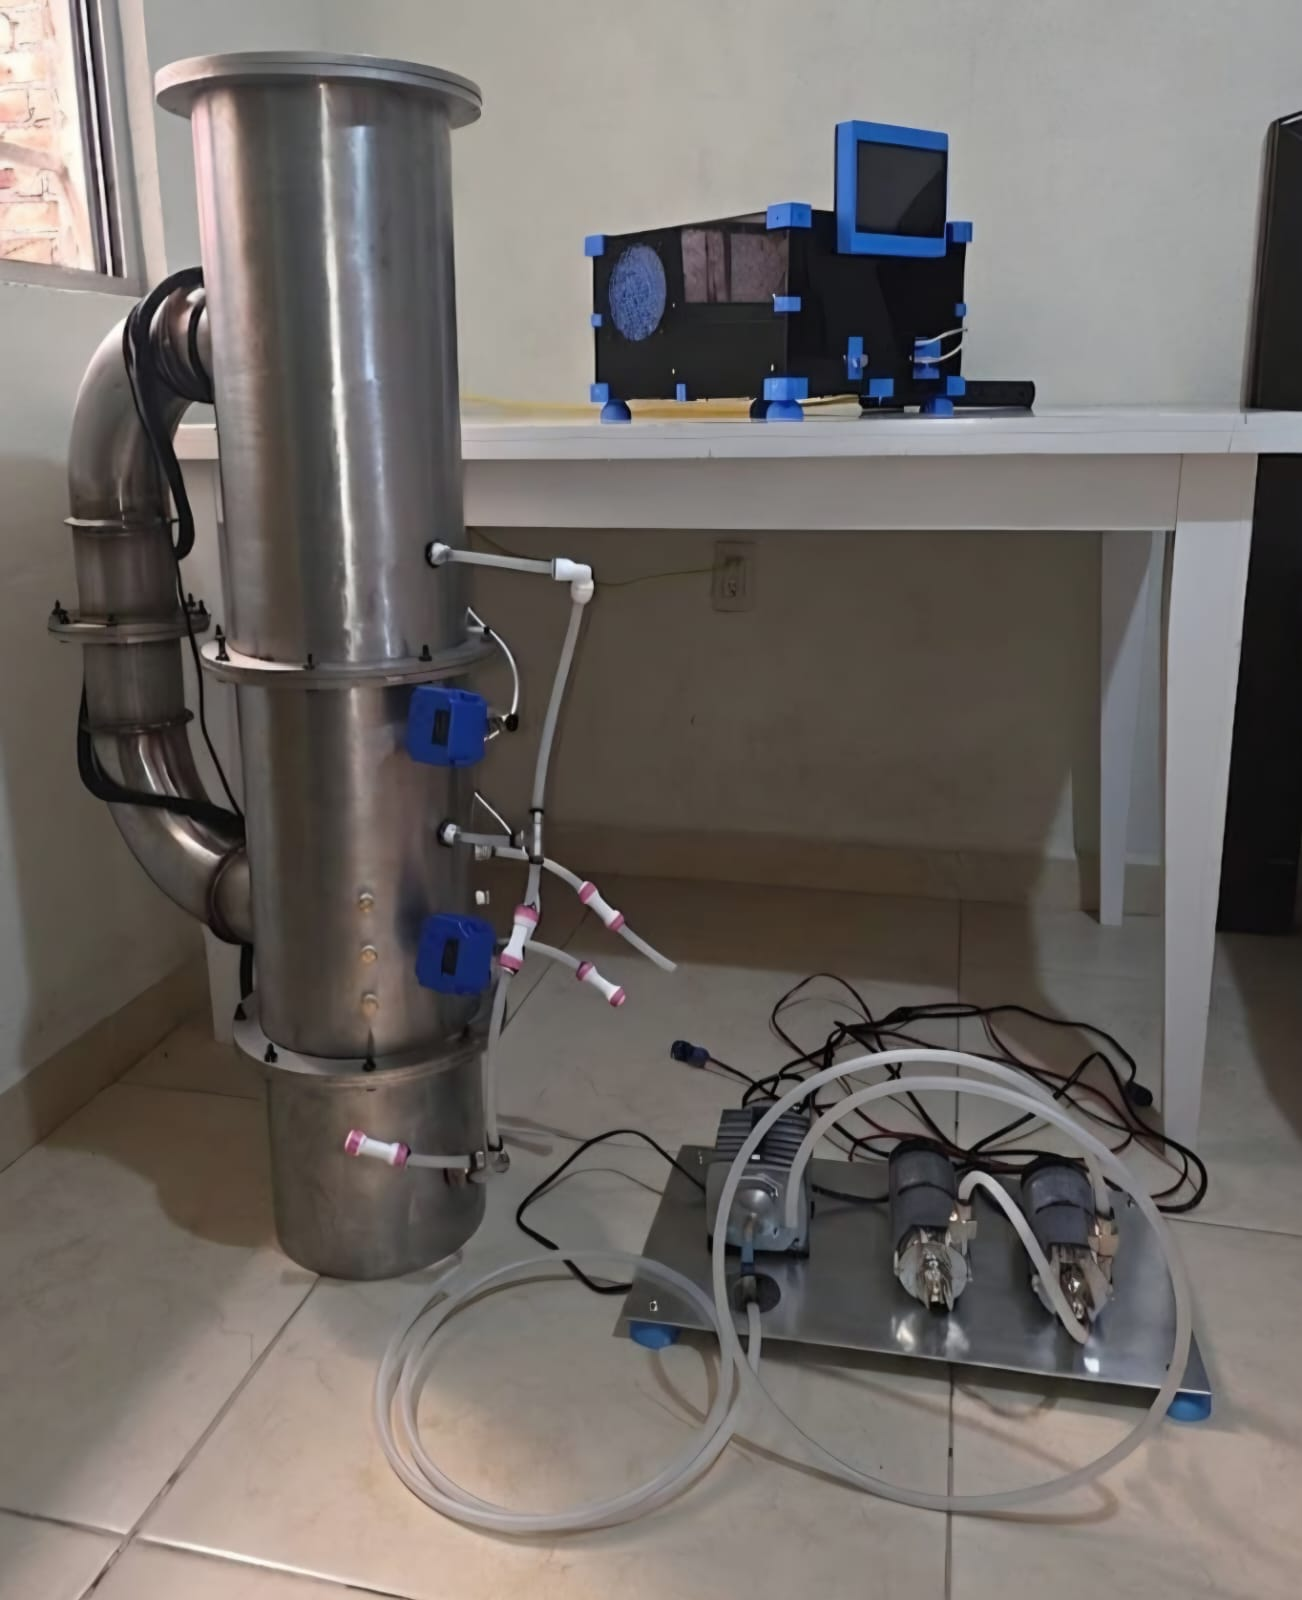
\includegraphics[width=0.65\textwidth]{Figuras/sistema_completo}
  \caption{Sistema completo del biorreactor.}
  \label{fig:sistema_completo}
\end{figure}

% ---------------------------------------------------------------
\section{Sistema de control de pH}
% ---------------------------------------------------------------

\subsection{Calibración del sensor de pH}

Para corroborar el funcionamiento del sensor RK500-12 y asegurar la exactitud
de las mediciones, se realizó una calibración de tres puntos mediante los
comandos definidos en el protocolo de comunicación Modbus del sensor.
Se utilizaron soluciones de referencia con valores de pH de 4, 7 y 10. Posterior
a la calibración, las lecturas del sensor reportaron un error máximo de
$\pm 0.1$~unidades de pH con respecto a la sustancia de referencia, cumpliendo
la resolución de 0.01~pH especificada por el fabricante. El error medio
registrado fue de $+0.088$~pH en buffer 4.0, $+0.058$~pH en buffer 7.0 y
$+0.030$~pH en buffer 10.0. Adicionalmente, la prueba de estabilidad en reposo
sobre 20 muestras arrojó una desviación estándar de $\sigma = 0.007$~pH,
bien por debajo del umbral de $0.05$~pH establecido como criterio de aceptación.
Los registros detallados de estas pruebas se encuentran en el
Anexo~\ref{ap:plan_pruebas_ph} (pruebas PH-02 a PH-05).

% ---------------------------------------------------------------
\subsection{Caracterización del comportamiento de pH}

Con el objetivo de definir la magnitud de la acción de control y justificar el
diseño asimétrico de los conjuntos difusos, se caracterizó experimentalmente
el comportamiento del medio ante la adición controlada de sustancia
neutralizadora.

Se simuló el medio de cultivo previo al ingreso del hongo utilizando una solución
compuesta por 8.5~g de sal por litro de agua, escalando el experimento a un
volumen reducido por practicidad pero respetando las proporciones del biorreactor.
El pH inicial de este medio se registró en 7.93. Posteriormente, se acidificó el
medio hasta un pH de 3.97 con ácido acético (vinagre) para emular el
comportamiento del metabolismo propio del organismo.

Se tomaron 301 muestras registrando el cambio de pH resultante de la adición
de volúmenes controlados de sustancia neutralizadora. En eventos clave se
realizaron mediciones de control con tiras indicadoras de pH como referencia
adicional.

La Figura~\ref{fig:curva_ph} muestra el cambio del pH en función de la cantidad de sustancia
estabilizadora aplicada, así como la ganancia registrada para cada zona
experimental.

\begin{figure}[H]
  \centering
  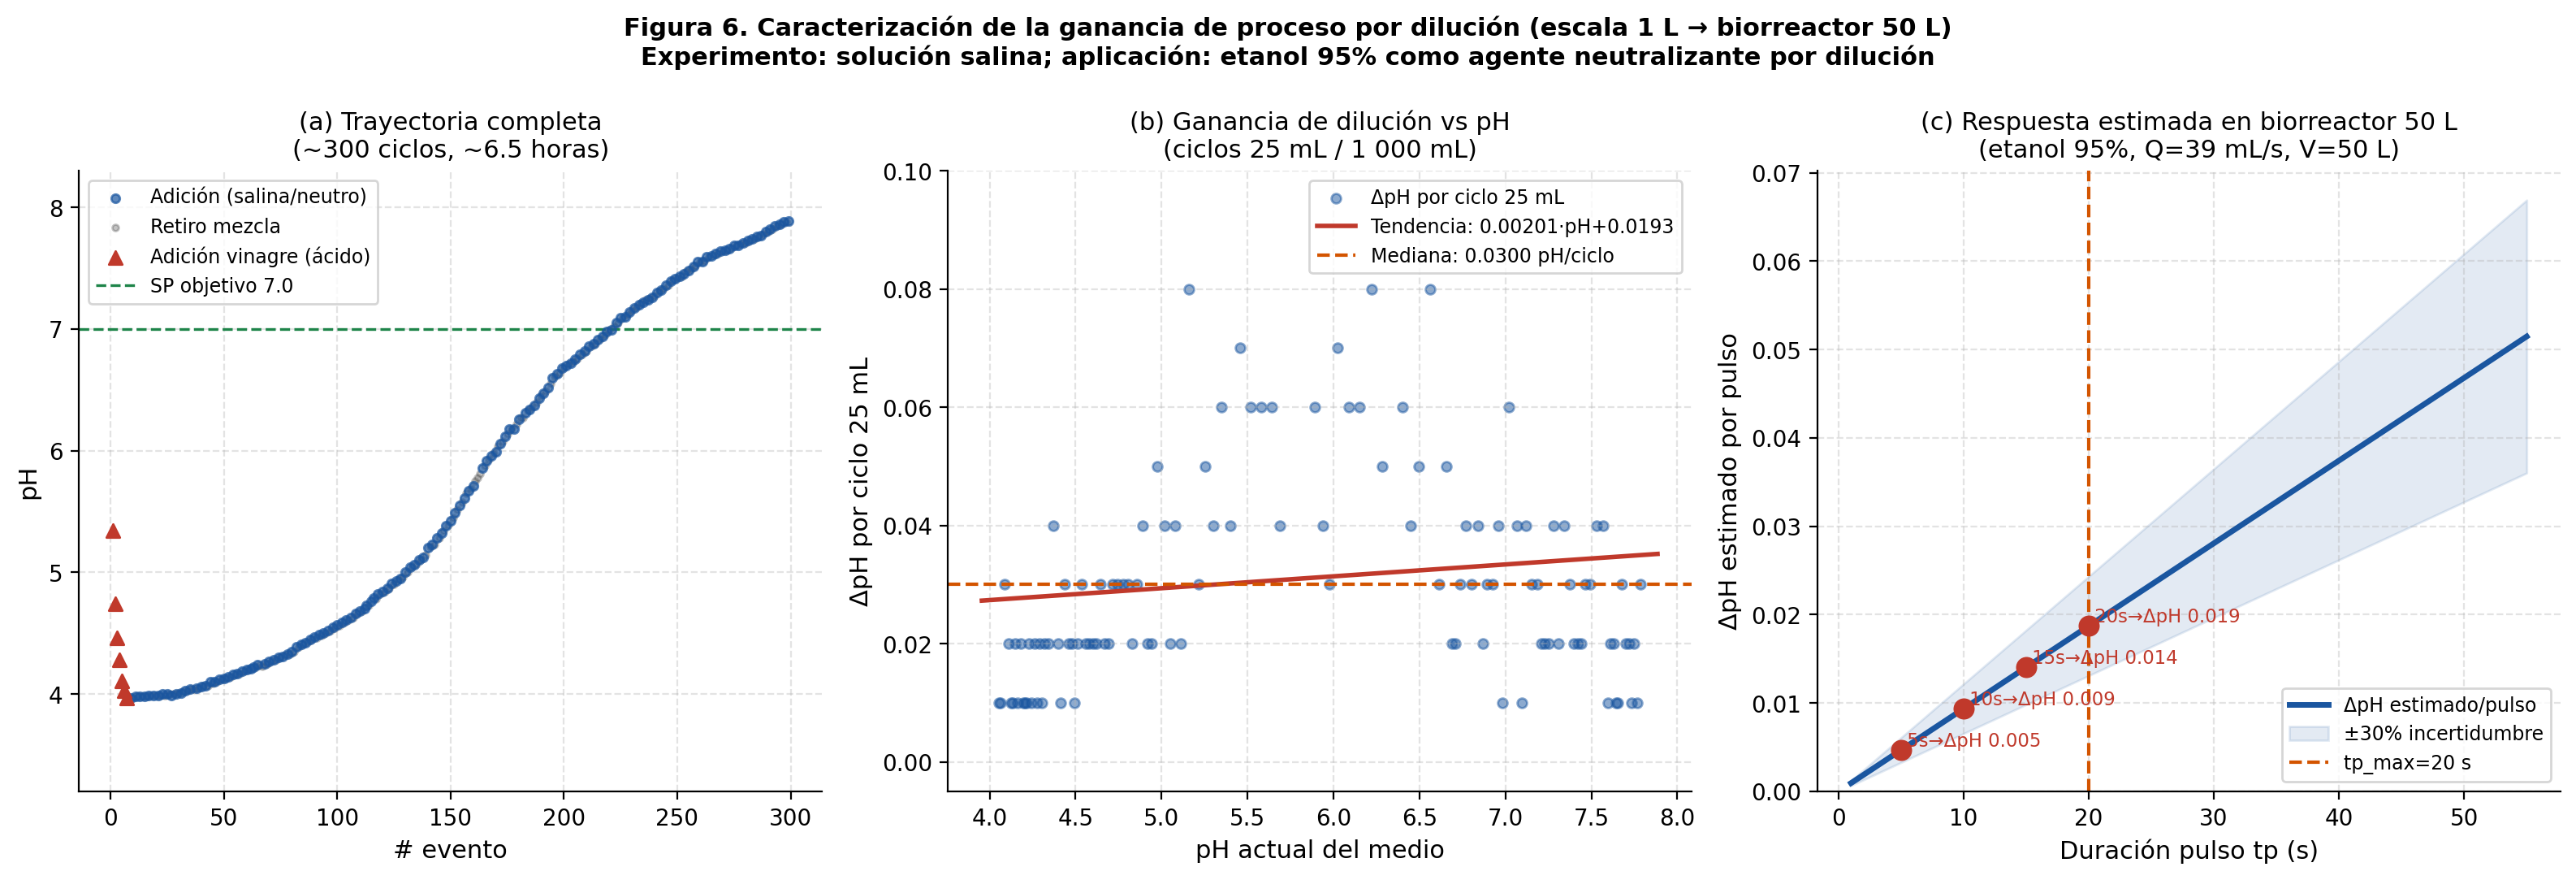
\includegraphics[width=\textwidth]{Figuras/fig_ganancia_proceso.png}
  \caption{Caracterización de la ganancia de proceso por dilución
           (escala 1~L $\to$ biorreactor 50~L). (a)~Trayectoria completa
           ($\approx$300 ciclos, $\approx$6.5~h). (b)~Ganancia por ciclo
           ($\Delta$pH/25~mL) en función del pH actual: mediana
           $\approx 0.030$~pH/ciclo. (c)~Respuesta estimada en biorreactor
           50~L: $\Delta$pH/pulso vs.\ duración del pulso a $Q=39$~mL/s.}
  \label{fig:curva_ph}
\end{figure}

Los datos capturados evidenciaron una ganancia relativamente constante en la
zona de operación normal ($4 < \text{pH} < 7$, ganancia mediana
$\approx 0.030$~pH/ciclo), con mayor dispersión en la zona muy ácida.
El panel~(c) confirma la relación lineal entre el tiempo de pulso y el
cambio de pH, validando el supuesto de bomba a caudal constante ($Q=39$~mL/s)
con $\Delta$pH$_\text{máx} \approx 0.06$~pH para $t_\text{pulso}=20$~s.
Este resultado justifica el diseño del controlador difuso con un universo de
salida de $[0, 20]$~s y el uso de conjuntos asimétricos para los errores más grandes.

% ---------------------------------------------------------------
\subsection{Tiempo de mezclado}

Con el objetivo de analizar las propiedades de mezclado del biorreactor
construido y determinar el tiempo de muestreo adecuado para el lazo de control,
se realizó una prueba de escalón consistente en la adición de un volumen definido
de vinagre al sistema. El pH fue registrado de forma continua hasta su
estabilización.

Empleando el criterio de estabilización al 95\%, utilizado convencionalmente en
procesos biológicos y químicos, la prueba arrojó un tiempo de estabilización
de \textbf{130~s}. La Figura~\ref{fig:mezclado_ph} muestra los valores de pH capturados durante esta
prueba.

\begin{figure}[H]
  \centering
  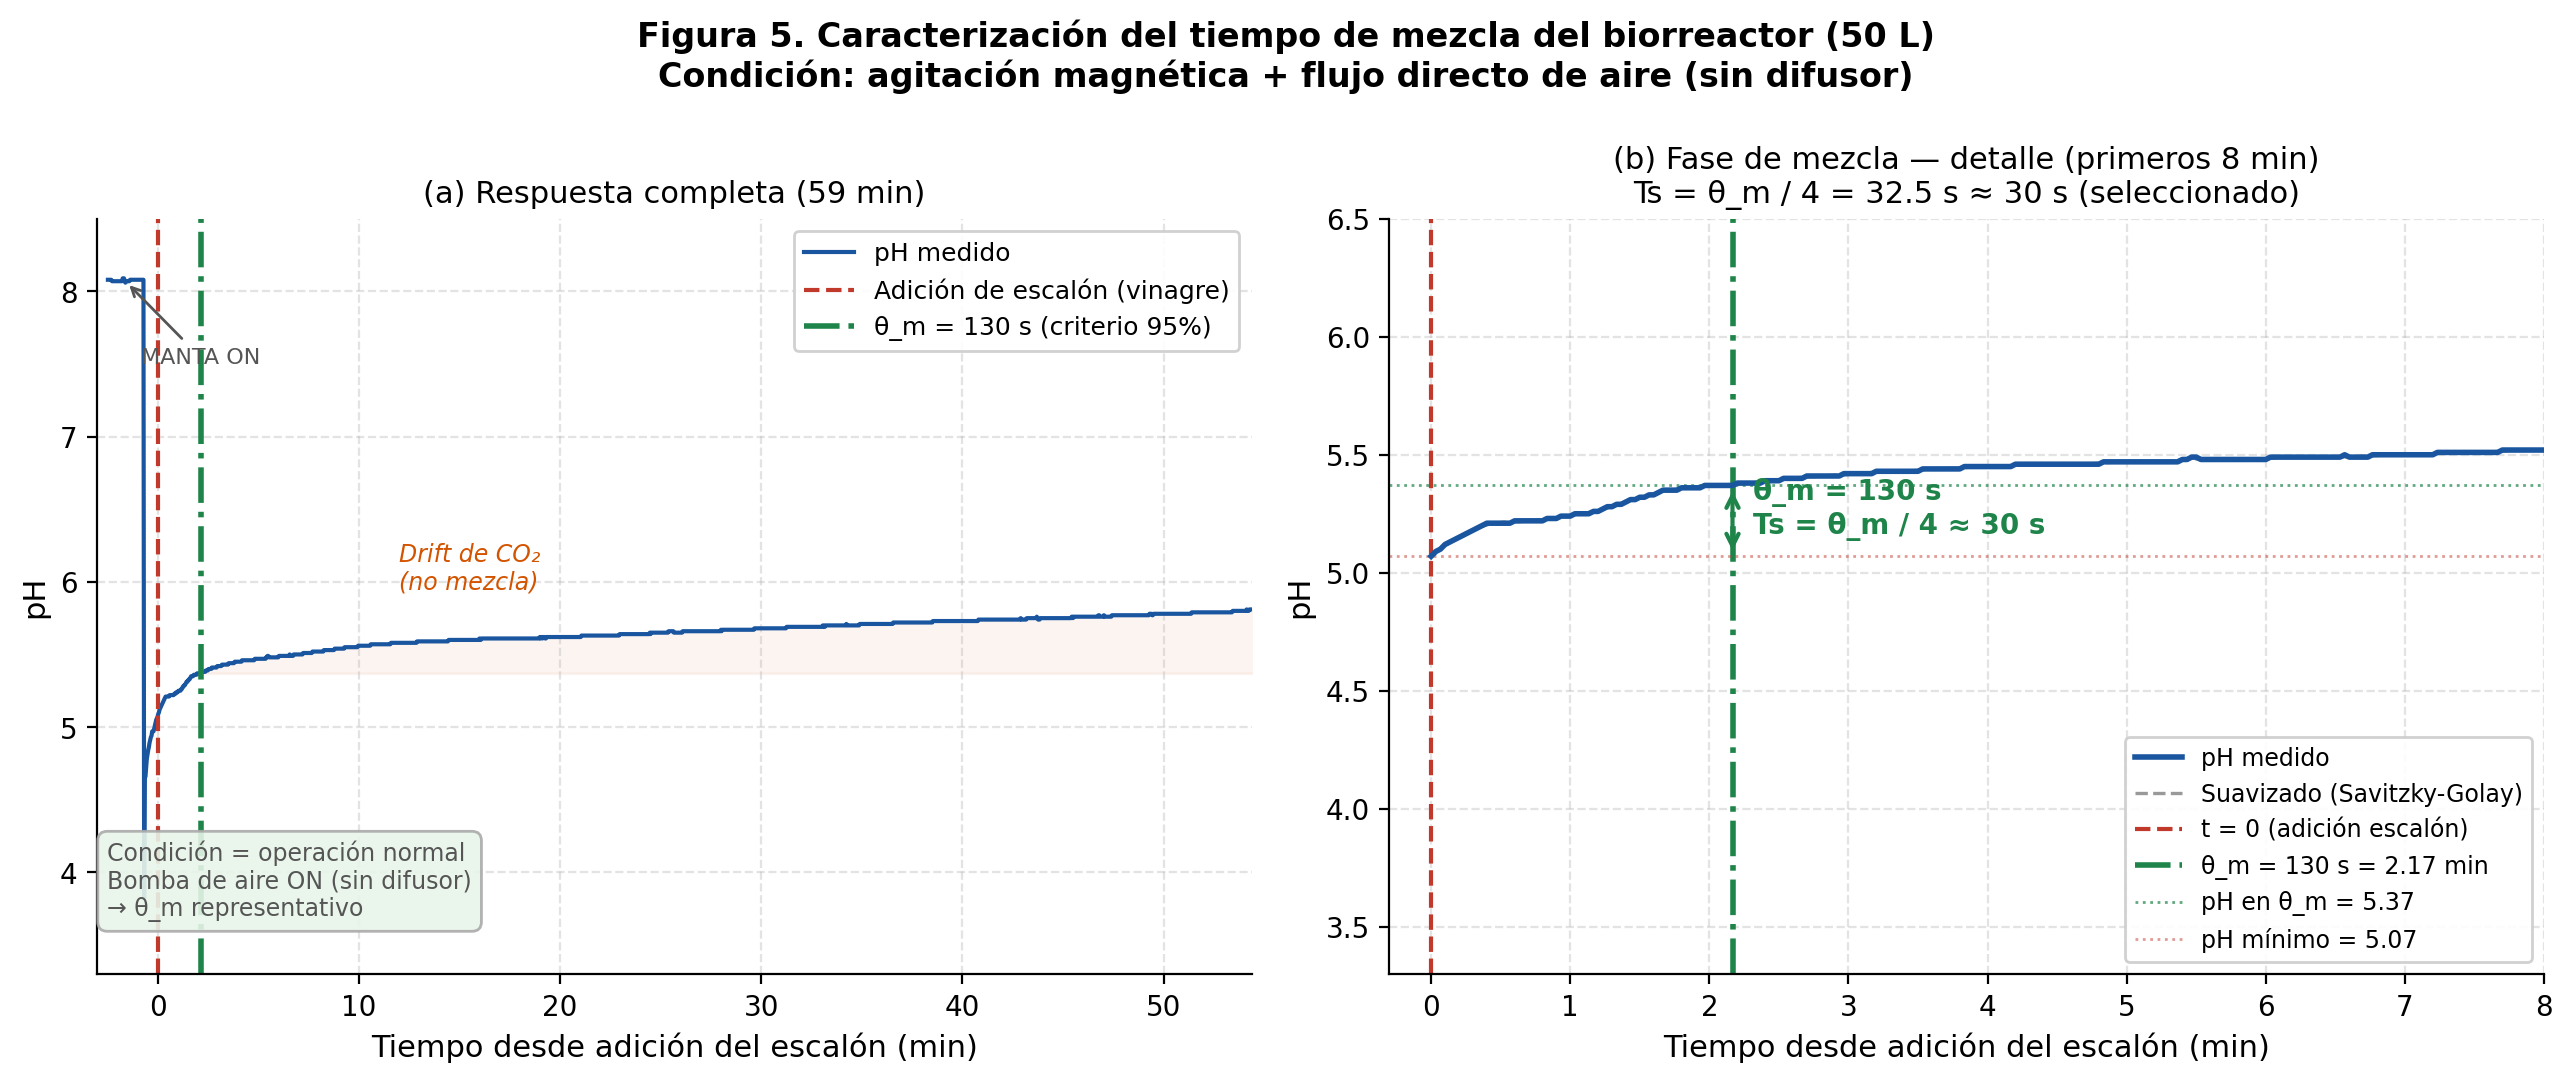
\includegraphics[width=\textwidth]{Figuras/fig_tiempo_mezcla_tesis.png}
  \caption{Caracterización del tiempo de mezcla del biorreactor (50~L).
           (a)~Respuesta completa (59~min) tras adición de escalón de vinagre
           con agitación magnética y flujo directo de aire (sin difusor).
           (b)~Detalle de los primeros 8~min: $\theta_m = 130$~s (criterio
           95\%), $T_s = \theta_m/4 \approx 32.5$~s; valor seleccionado
           $T_s = 30$~s.}
  \label{fig:mezclado_ph}
\end{figure}

Este resultado llevó a establecer un tiempo entre muestras de $T_s = 30$~s,
valor redondeado al alza para garantizar que cada lectura sea significativa
y útil para la toma de decisiones de control.

% ---------------------------------------------------------------
\subsection{Caudal promedio de la bomba neutralizadora}

Para determinar el caudal real de la bomba utilizada en el sistema de control
de pH, se realizó una prueba de llenado del tanque hasta su volumen de
operación máximo de 55~L. El tiempo de llenado registrado fue de 1\,409~s,
con lo que el caudal promedio queda determinado por:

\begin{equation}
  Q = \frac{V}{t} = \frac{55\,000~\text{mL}}{1\,409~\text{s}} \approx 39~\text{mL/s}
\end{equation}

Este valor fue empleado para establecer la relación entre el tiempo de pulso
$t_{\text{pulso}}$ definido por el controlador difuso y el volumen de neutralizador
entregado al sistema en cada ciclo de control (véase Tabla~\ref{tab:mf_salida}).

% ---------------------------------------------------------------
\subsection{Validación del controlador difuso}

El controlador difuso de pH fue validado en lazo cerrado con la interfaz para pruebas
\texttt{prueba\_visual\_ph.py} (Anexo~\ref{ap:codigo_prueba_ph}). Para simular el metabolismo del hongo, el
medio se acidificó con ácido acético hasta distintos valores iniciales de pH.

\subsubsection*{Verificación de la inferencia (lazo abierto)}

Las pruebas de inferencia en lazo abierto (FZ-01 a FZ-05) confirmaron el
comportamiento esperado de los cinco conjuntos difusos. Con errores dentro de la
banda muerta ($e \leq 0.1$~pH) el controlador emitió $t_\text{pulso} = 0$~s en todos
los casos. Para los conjuntos PE, ME y GE los tiempos de pulso medidos fueron de
$9.2$--$10.4$~s, $13.6$--$14.5$~s y $17.8$--$18.6$~s respectivamente, dentro
de los rangos de aceptación definidos. El conjunto MG ($e \geq 0.8$~pH) produjo
exactamente $t_\text{pulso} = 20.0$~s (saturación directa) en los tres ensayos.

\subsubsection*{Desempeño en lazo cerrado}

Las pruebas FZ-06 a FZ-08 evaluaron la respuesta del sistema en lazo cerrado con
SP = 7.0~pH. Los resultados principales se resumen a continuación:

\begin{itemize}
  \item \textbf{Convergencia (FZ-06):} Partiendo de pH inicial 6.84, 5.99 y 5.82,
  el sistema convergió al SP en 7, 11 y 18~minutos respectivamente,
  alcanzando pH $\in [\text{SP} \pm 0.04]$ en tres ciclos consecutivos.
  \item \textbf{Sobreimpulso (FZ-07):} El sobreimpulso máximo observado fue de
  $0.06$~pH, muy por debajo del límite de $0.5$~pH.
  \item \textbf{Rechazo de perturbación (FZ-08):} Ante perturbaciones por burbujeo
  activo, el controlador recuperó el SP en $\leq 3$ ciclos de control ($\leq 90$~s).
\end{itemize}

Finalmente, la prueba de integración continua (INT-01) confirmó operación estable
durante 30~minutos con pH mantenido en $[6.7, 7.1]$ y cero fallas de comunicación
por RS-485 ni I$^2$C. El plan de pruebas completo con 29 casos organizados en
categorías de sensor de pH, sensor de nivel, actuadores, inferencia difusa, lazo
cerrado, gestión de nivel, seguridad e integración se detalla en el
Anexo~\ref{ap:plan_pruebas_ph}.

La Figura~\ref{fig:control_ph_pruebas} muestra las curvas de pH y las acciones de
control (tiempo de pulso por ciclo) para las cinco pruebas de validación en lazo
cerrado, y la Figura~\ref{fig:control_ph_metricas} resume el tiempo de
establecimiento y el error en estado estable de cada una.

\begin{figure}[H]
  \centering
  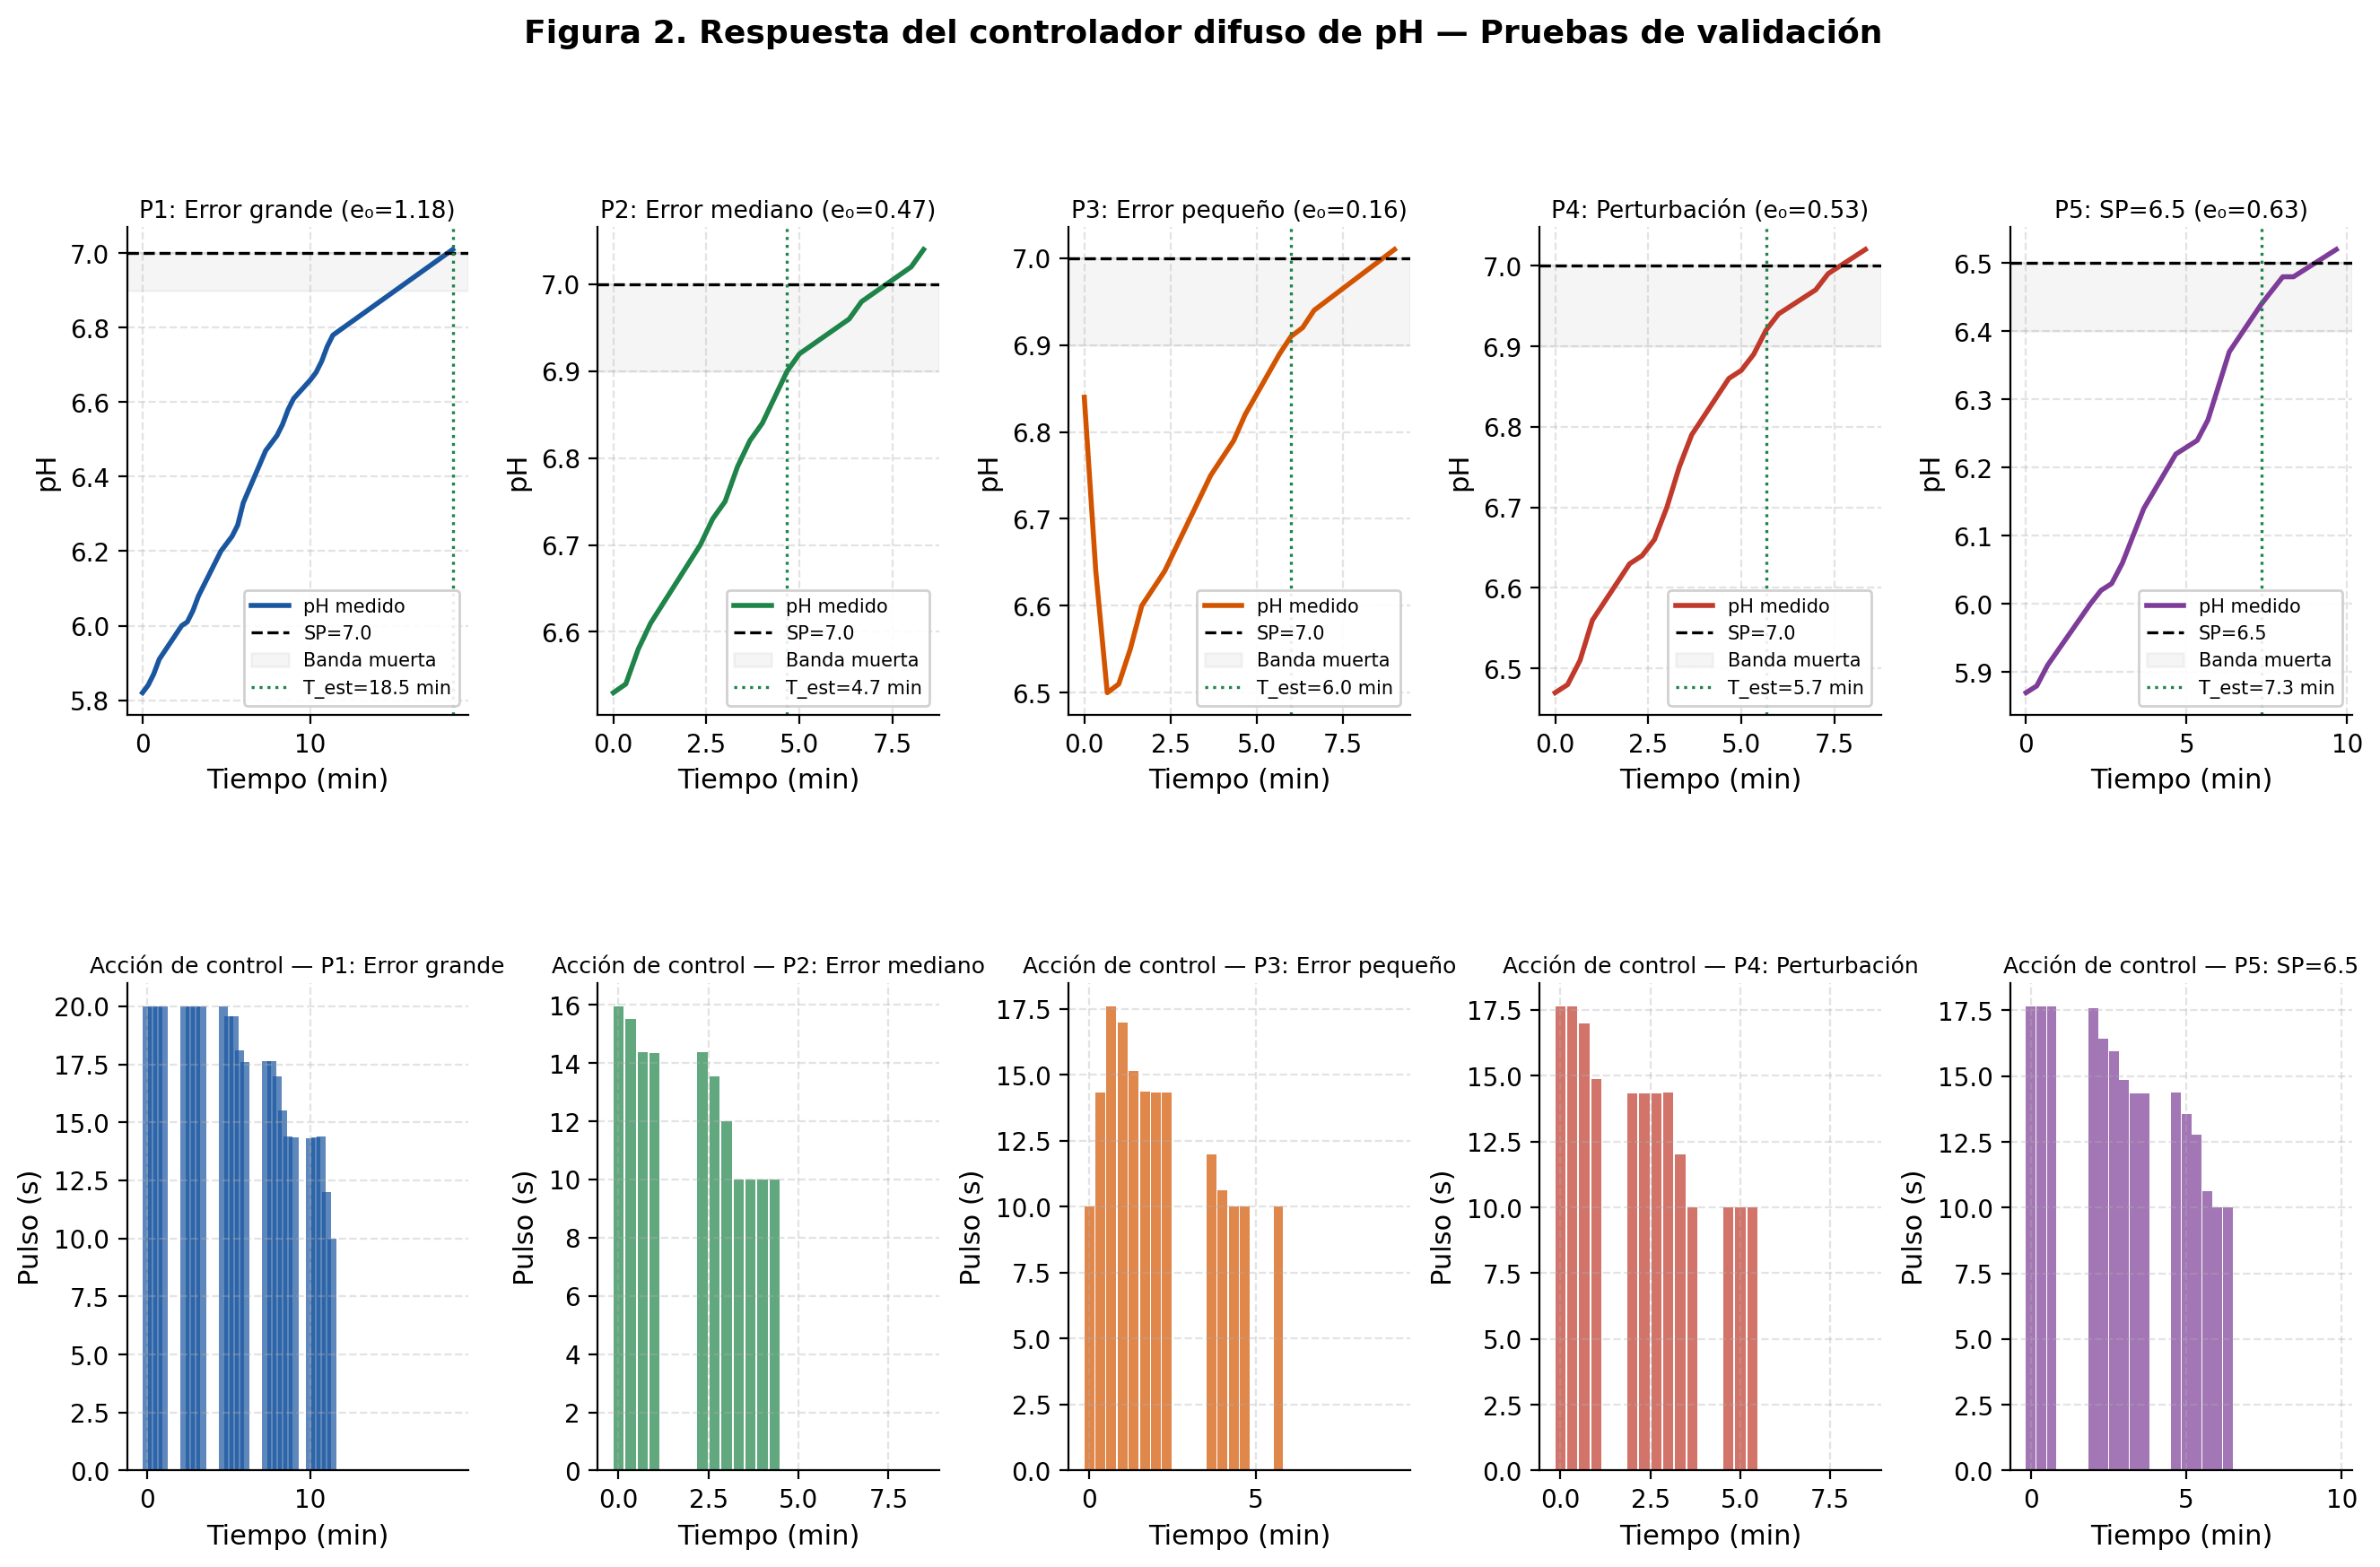
\includegraphics[width=\textwidth]{Figuras/fig_control_ph_pruebas.png}
  \caption{Respuesta del controlador difuso de pH en cinco escenarios de validación.
           Fila superior: pH medido y SP = 7.0~pH (excepto P5: SP = 6.5~pH).
           Fila inferior: tiempo de pulso emitido por el controlador en cada ciclo
           de muestreo ($T_s = 30$~s). Los valores de error inicial
           $e_0$ son 1.18, 0.47, 0.16, 0.53 y 0.63~pH para P1--P5
           respectivamente.}
  \label{fig:control_ph_pruebas}
\end{figure}

\begin{figure}[H]
  \centering
  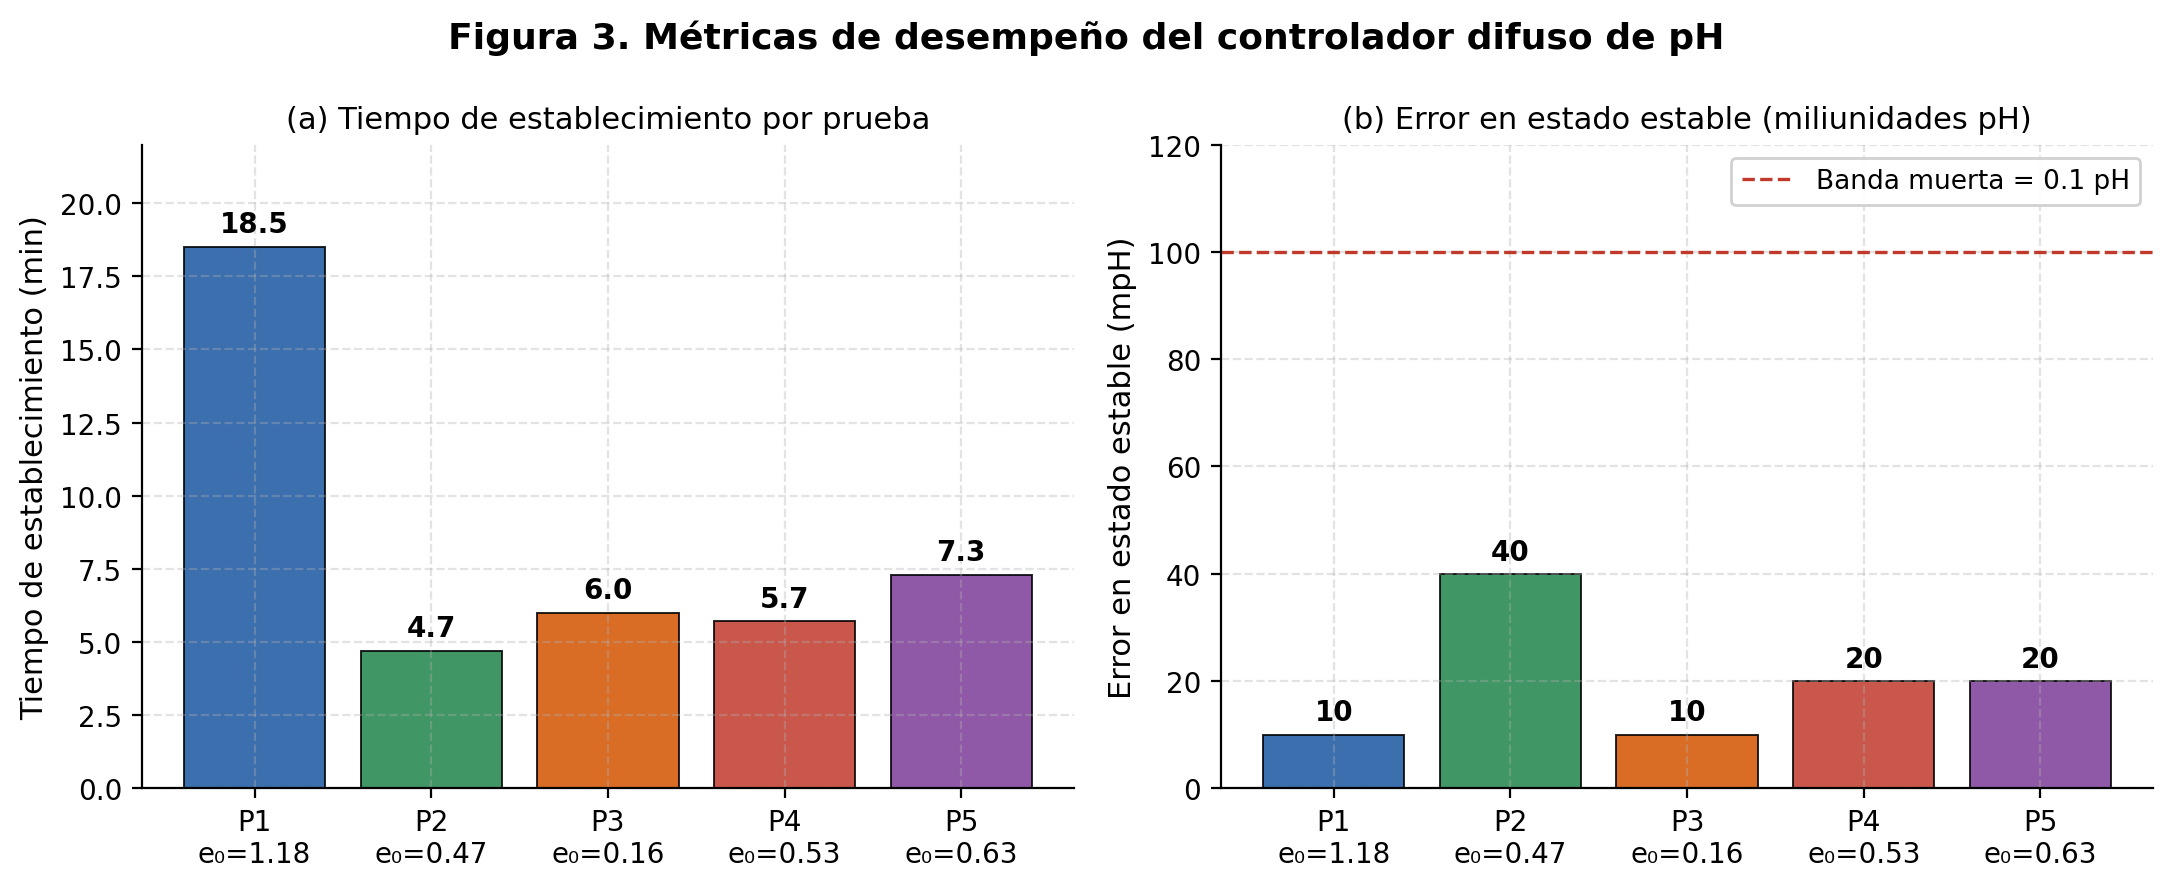
\includegraphics[width=\textwidth]{Figuras/fig_control_ph_metricas.png}
  \caption{Métricas de desempeño del controlador difuso de pH.
           (a)~Tiempo de establecimiento por prueba: rango de 4.7 a 18.5~min.
           (b)~Error en estado estable: máximo de 40~mpH (P2), todos por
           debajo de la banda muerta de 100~mpH.}
  \label{fig:control_ph_metricas}
\end{figure}

% ---------------------------------------------------------------
\section{Sistema de control de nivel}
% ---------------------------------------------------------------

\subsection{Inicialización y calibración del sensor XM125}

La inicialización por I$^2$C del sensor de nivel XM125 se verificó exitosamente
(prueba NV-01). Sin embargo, la calibración en estado vacío (prueba NV-02) reveló
una limitación de hardware: el sensor no reporta mediciones válidas por debajo del
22\,\% de nivel de llenado, equivalente a aproximadamente 805\,mm de distancia
desde la tapa. Este umbral se estableció como el punto mínimo de operación confiable.

La calibración en estado lleno (NV-03) arrojó una distancia estable de
$151 \pm 2$~mm en tres repeticiones, dentro del criterio de $\pm 5$~mm. La
exactitud del porcentaje de nivel (NV-04) se evaluó en cuatro puntos de la escala:
el error máximo observado fue del 1.0\,\% (95\,\% real leído como 96.0\,\%), bien por
debajo del límite del 5\,\%. El filtro de picos del nivel (NV-05) respondió
correctamente ante 5 perturbaciones artificiales en las tres repeticiones, sin
producir saltos en la señal de nivel presentada al controlador. Los registros
completos se encuentran en el Anexo~\ref{ap:plan_pruebas_ph} (pruebas NV-01 a NV-05).

% ---------------------------------------------------------------
\subsection{Gestión de nivel y auto-vaciado}

El lazo de histéresis para la gestión de nivel fue validado mediante las pruebas
LV-01 a LV-03. La electroválvula de drenado (CH8) respondió dentro de los
$\leq 2$~s tras superar el umbral del 99\,\% de nivel (criterio $\leq 3$~s), y el
cierre automático ocurrió consistentemente al descender a $96.0 \pm 0.1$\,\%
(criterio $96 \pm 1$\,\%). Durante el vaciado, la inhibición del control de pH fue
efectiva en el 100\,\% de los ciclos registrados en las tres repeticiones,
garantizando que no se añada neutralizador mientras el nivel desciende. Los
registros detallados se encuentran en el Anexo~\ref{ap:plan_pruebas_ph}
(pruebas LV-01 a LV-03).

% ---------------------------------------------------------------
\section{Sistema de control de luz}
% ---------------------------------------------------------------

\subsection{Caracterización de la respuesta del actuador luminoso}

Para establecer la relación entre la señal de control y la iluminancia
entregada en el interior del biorreactor, se realizó un barrido del ciclo de
trabajo del PWM desde 0\,\% hasta 100\,\% en pasos de 10\,\%, utilizando el
foco encapsulado alimentado a 12\,V con una resolución de 12~bits (rango
0--4095). El sensor de luz (luxómetro) se colocó en el fondo del tanque vacío,
registrando la iluminancia en el punto más alejado de la fuente.

Las Figuras~\ref{fig:pwm_barrido_completo} y~\ref{fig:pwm_barrido_zoom}
muestran el registro temporal del barrido a escala completa y con detalle
de la zona de mayor intensidad, respectivamente.

\begin{figure}[H]
  \centering
  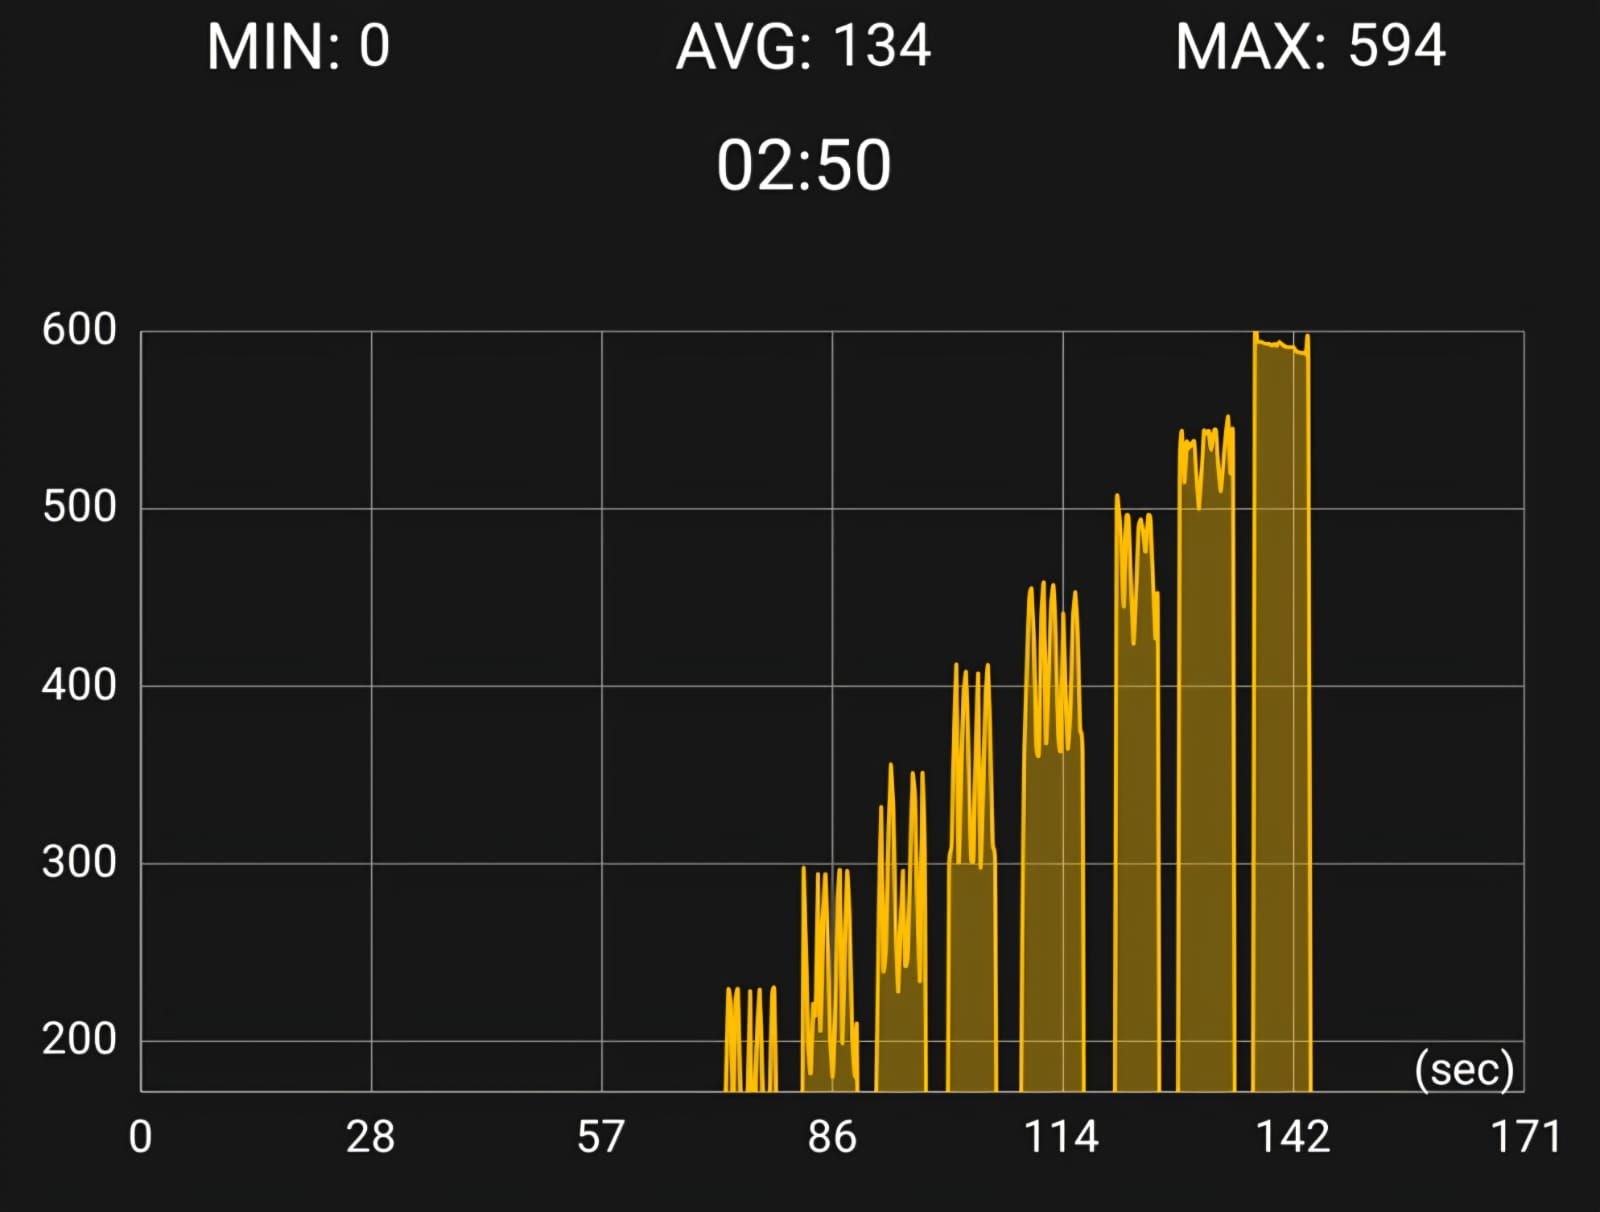
\includegraphics[width=0.82\textwidth]{Figuras/todo.jpeg}
  \caption{Barrido completo del PWM (0--100\,\%). La iluminancia aumenta de
           forma escalonada; cada peldaño corresponde a un incremento del
           10\,\% en el ciclo de trabajo. MIN\,=\,0\,Lux,
           AVG\,=\,134\,Lux, MAX\,=\,597\,Lux.}
  \label{fig:pwm_barrido_completo}
\end{figure}

\begin{figure}[H]
  \centering
  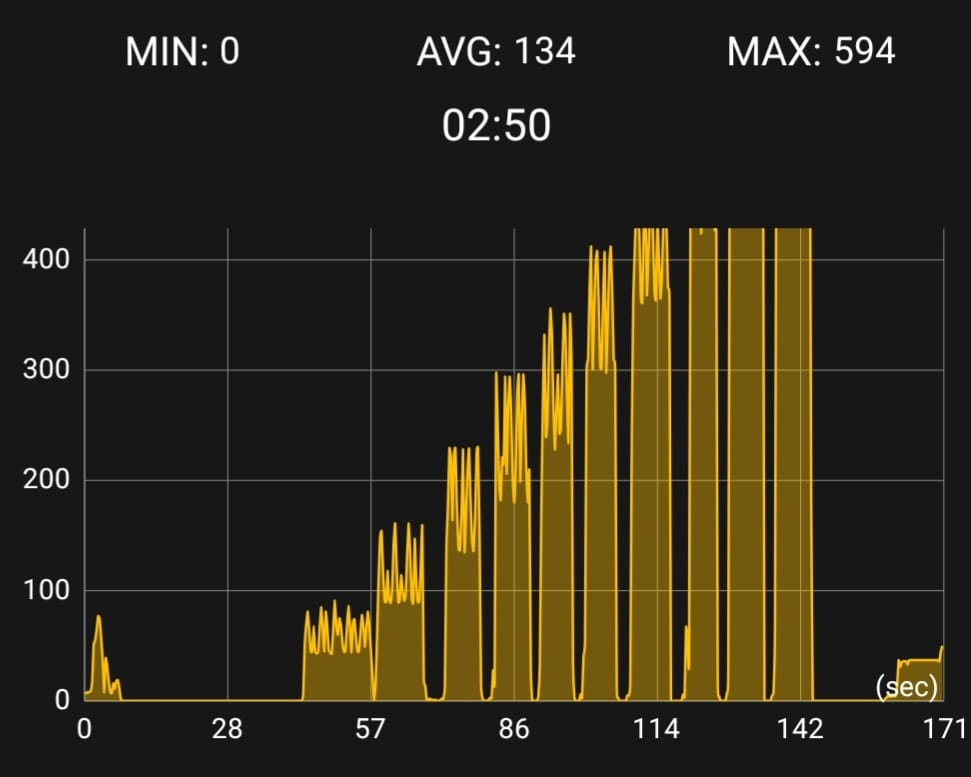
\includegraphics[width=0.82\textwidth]{Figuras/recortado.jpeg}
  \caption{Acercamiento del barrido (zona de 200--600\,Lux), donde se
           aprecian con mayor claridad los peldaños de cada incremento del
           ciclo de trabajo.}
  \label{fig:pwm_barrido_zoom}
\end{figure}

La Tabla~\ref{tab:pwm_niveles} resume la iluminancia media registrada en
cada nivel del barrido.

\begin{table}[H]
\centering
\caption{Iluminancia medida en cada nivel del barrido PWM.}
\label{tab:pwm_niveles}
\renewcommand{\arraystretch}{1.3}
\small
\adjustbox{max width=\textwidth}{%
\begin{tabular}{@{} r r r @{}}
\toprule
\textbf{PWM (\%)} & \textbf{Valor (0--4\,095)} & \textbf{Iluminancia (Lux)} \\
\midrule
  0 &     0 &   0 \\
 10 &   410 &  82 \\
 20 &   819 & 159 \\
 30 & 1\,229 & 230 \\
 40 & 1\,638 & 295 \\
 50 & 2\,048 & 352 \\
 60 & 2\,457 & 408 \\
 70 & 2\,867 & 456 \\
 80 & 3\,276 & 497 \\
 90 & 3\,686 & 545 \\
100 & 4\,095 & 597 \\
\bottomrule
\end{tabular}
}
\end{table}

\subsection{Ajuste lineal y punto de operación}

La Figura~\ref{fig:pwm_curva_ajuste} presenta los once puntos del barrido
junto con la recta de regresión por mínimos cuadrados. La relación entre
el ciclo de trabajo $d$ (en porcentaje) y la iluminancia $E$ (en Lux) es
aproximadamente lineal en todo el rango:

\begin{equation}
  E \approx 5.83 \times d + 38 \qquad (R^2 = 0.988)
  \label{eq:pwm_lux}
\end{equation}

Expresada sobre la escala de 12~bits ($D$, de 0 a 4\,095):
$E \approx 0.142 \times D + 38$. La ecuación inversa permite calcular el
ciclo de trabajo necesario para alcanzar una iluminancia objetivo:

\begin{equation}
  d \approx \frac{E - 38}{5.83}
  \label{eq:lux_pwm}
\end{equation}

\begin{figure}[H]
  \centering
  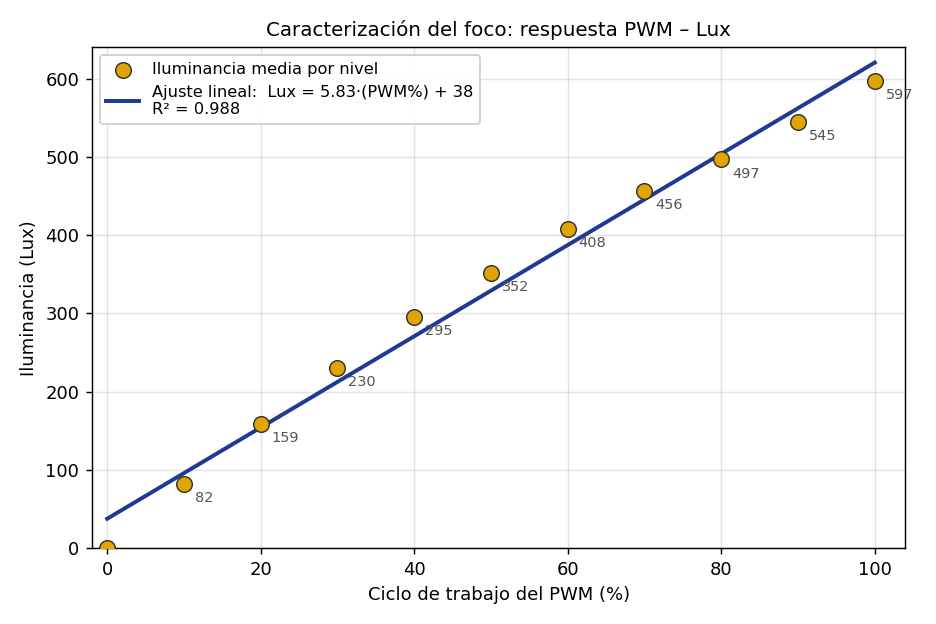
\includegraphics[width=0.85\textwidth]{Figuras/pwm_curva_ajuste.png}
  \caption{Iluminancia media por nivel en función del ciclo de trabajo del PWM
           y recta de ajuste lineal ($R^2 = 0.988$). Los datos confirman un
           comportamiento lineal en todo el rango de 0 a 597\,Lux.}
  \label{fig:pwm_curva_ajuste}
\end{figure}

El coeficiente $R^2 = 0.988$ confirma la linealidad del actuador a lo largo
de todo el rango. El valor de referencia medido en condiciones naturales del
espacio de trabajo es de aproximadamente 478\,Lux, equivalente a un ciclo de
trabajo del $d \approx 75\,\%$ (valor de 12~bits $\approx 3\,072$), que
puede fijarse directamente por software.

% ---------------------------------------------------------------
\section{Sensor de oxígeno disuelto}
% ---------------------------------------------------------------

\subsection{Calibración del sensor RK500-04}

El sensor de oxígeno disuelto RK500-04 requiere una calibración de dos puntos
para fijar su curva de respuesta: un punto de cero oxígeno y un punto de
saturación al aire. La comunicación se realizó mediante Modbus RTU sobre
UART (\texttt{/dev/serial0}, 9600~baud, esclavo dirección~10), leyendo
continuamente los registros~0--5, que contienen tres valores \texttt{float32}
en formato big-endian: OD (mg/L), saturación (\%) y temperatura (°C).

\subsubsection*{Punto de saturación (calibración al aire)}

Se expuso el electrodo al aire ambiente durante 180~s hasta estabilizar la
lectura. El oxígeno disuelto en equilibrio con la atmósfera a nivel del mar y
temperatura ambiente se encuentra en el rango de 8--9~mg/L; el sensor reportó
valores de \textbf{7.0--9.0~mg/L}, consistentes con este intervalo. El comando
de calibración se envía escribiendo el valor~1 en el registro~0x1A (26 decimal)
del sensor.

\subsubsection*{Punto cero (calibración en agua desoxigenada)}

Se preparó agua hervida durante 20~minutos para eliminar el oxígeno disuelto
y se sumergió el electrodo. Tras esperar la estabilización, la primera lectura
fue de 0.1--0.6~mg/L y la segunda medición arrojó \textbf{0.21~mg/L},
confirmando la eliminación casi total del oxígeno. El comando de calibración
cero se envía escribiendo el valor~1 en el registro~0x1C (28 decimal).

\subsubsection*{Resultado}

Con ambos puntos almacenados en la memoria interna del sensor, las lecturas
posteriores en agua con burbujeo activo se mantuvieron dentro del rango
esperado para el medio de cultivo. El script de calibración utilizado se
incluye en el Anexo~\ref{ap:codigo_prueba_ph} junto con el modo de lectura
continua que decodifica los registros Modbus a valores físicos.
